\documentclass[11pt]{article}

\usepackage[margin=1in]{geometry}
\usepackage{amsmath, amssymb}
\usepackage{graphicx}
\usepackage{booktabs}
\usepackage{hyperref}
\usepackage{xcolor}
\usepackage{caption}
\usepackage{subcaption}
\usepackage{listings}

\hfuzz=\maxdimen

\graphicspath{{../../figures/iterative_probe/}}

\newcommand{\lcq}[1]{\textcolor{red}{#1}}
\newcommand{\code}[1]{\texttt{#1}}

\lstset{
  basicstyle=\ttfamily\small,
  breaklines=true,
  frame=single,
  language=Python,
  keywordstyle=\color{blue},
  commentstyle=\color{gray},
}

\title{Iterative Linear Probing and Counterfactual Importance:\\
       Redundancy in Belief-State Representations}
\author{Claude \& C.~L.}
\date{\today}

\begin{document}
\maketitle
\tableofcontents
\bigskip

%----------------------------------------------------------------------
\section{Introduction}
\label{sec:intro}
%----------------------------------------------------------------------

Previous probing experiments on transformers trained on Hidden Markov Model (HMM) data have established that the residual stream encodes a high-fidelity linear image of the Bayesian belief state (the posterior distribution over hidden states given the observed token history).  A natural follow-up question is: \emph{how many independent copies} of this belief state does the network store, and \emph{which copies matter} for the model's actual next-token predictions?

These questions bear on two distinct aspects of the representation:

\begin{enumerate}
  \item \textbf{Redundancy.}  A 64-dimensional residual stream need only devote 2 dimensions to represent the Mess3 belief state (which lives on a 2-simplex).  If the network stores multiple independent copies, this tells us something about how superposition and redundancy interact in small transformers---and whether the network ``wastes'' capacity or exploits it for robustness.
  \item \textbf{Causal relevance.}  A subspace may be linearly decodable without being causally used by downstream layers.  Counterfactual ablation (replacing a subspace's projection with its mean) tests whether the model's output \emph{changes} when that information is erased, distinguishing representation from mere correlation.
\end{enumerate}

This report describes the \emph{iterative probing} algorithm and its application to a 4-layer, 64-dimensional, single-head transformer trained on the Mess3 process.

%----------------------------------------------------------------------
\section{Model and Process}
\label{sec:model}
%----------------------------------------------------------------------

The Mess3 process (\code{src/hmm.py}, class \code{Mess3Proc}) is a 3-state, 3-token HMM.  The model is a 4-layer HookedTransformer with $d_{\text{model}} = 64$, a single attention head ($d_{\text{head}} = 64$), MLP width 256, ReLU activations, and LayerNorm.  It was trained on 10M tokens with context length $n_{\text{ctx}} = 10$.  The model directory is:
\begin{center}
\code{models/mess3/20260306\_150920\_L4\_d64\_H1\_full\_LN/}
\end{center}

The belief state for Mess3 has 3 components summing to 1, so it lives on a 2-dimensional simplex embedded in $\mathbb{R}^3$.  A linear probe mapping $\mathbb{R}^{64} \to \mathbb{R}^3$ therefore has a coefficient matrix of shape $3 \times 64$ whose row space is generically 2-dimensional (or at most 3, depending on how the intercept interacts with the sum-to-one constraint).

%----------------------------------------------------------------------
\section{Algorithm}
\label{sec:algorithm}
%----------------------------------------------------------------------

\subsection{Iterative Probing}
\label{sec:iterative-probing}

The core idea is to repeatedly extract and remove the best linear predictor of the belief state from the activations, counting how many times this can be done before the residual signal drops below a significance threshold.

For each layer $\ell$:
\begin{enumerate}
  \item Let $X^{(0)} \in \mathbb{R}^{n \times 64}$ be the last-position residual-stream activations.
  \item At iteration $k$:
    \begin{enumerate}
      \item Fit a linear probe: $\hat{y} = X^{(k)} W^\top + b$, where $W \in \mathbb{R}^{3 \times 64}$.
      \item Evaluate test $R^2$.  If $R^2 < \tau$ (default $\tau = 0.05$), stop.
      \item Compute the SVD of $W = U \Sigma V^\top$.  Retain rows of $V^\top$ corresponding to singular values above a relative threshold ($\sigma_i / \sigma_0 > 10^{-3}$).  Call the retained rows $V_k \in \mathbb{R}^{r_k \times 64}$, where $r_k$ is the effective rank.
      \item Project out: $X^{(k+1)} = X^{(k)} - X^{(k)} V_k^\top V_k$.
    \end{enumerate}
  \item The number of iterations with $R^2 \geq \tau$ is the number of ``independent copies.''
\end{enumerate}

This is implemented in \code{src/iterative\_probe.py}, with the main entry points being \code{iterative\_probe\_single\_layer()} and \code{iterative\_probe\_all\_layers()}.  The function \code{extract\_subspace()} performs the SVD and rank thresholding; \code{project\_out\_subspace()} handles the orthogonal projection.  The algorithm reuses \code{fit\_probe\_with\_split()} from \code{src/linear\_probe.py} at each iteration to ensure a consistent 80/20 train/test split.

\paragraph{Why $R^2$ and not MSE?}
MSE depends on the scale of the targets, while $R^2$ is normalised.  Because the projected activations have shrinking variance with each iteration, MSE alone could be misleading; $R^2$ measures the fraction of target variance explained regardless of the activation scale.

\subsection{Counterfactual Importance via Mean Ablation}
\label{sec:counterfactual}

For each layer $\ell$ and each iteration-$k$ subspace $V_k$:
\begin{enumerate}
  \item Run the model cleanly to obtain reference log-probabilities $\log p_{\text{clean}}$ at the last token position.
  \item Intervene on the residual stream at layer $\ell$ using a \code{run\_with\_hooks} forward hook: project the activations onto $V_k$, replace the projection with its batch mean, and add back the residual.  Formally, if $a$ is the activation vector:
  \begin{equation}
    a' = a - V_k^\top V_k \, a + \mathbb{E}_{\text{batch}}[V_k^\top V_k \, a].
  \end{equation}
  \item Compute the KL divergence: $D_{\text{KL}}(p_{\text{clean}} \| p_{\text{ablated}})$, which measures how much the model's output distribution shifts when this subspace is erased.
  \item Also compute the cross-entropy change $\Delta\text{CE}$ as a secondary metric.
\end{enumerate}

This is implemented in \code{src/run\_iterative\_probe.py}, functions \code{ablate\_subspace()} and \code{compute\_counterfactual()}.  The ablation generalises the single-direction ablation in \code{archive/old\_src/ablation.py} to arbitrary-dimensional subspaces via the einsum-based projection \code{t.einsum("bsd,rd->bsr", actvs, subspace)}.

We additionally ablate each individual SVD direction within a subspace and the cumulative subspace (all iterations combined) to obtain finer-grained attribution.

%----------------------------------------------------------------------
\section{Results}
\label{sec:results}
%----------------------------------------------------------------------

The experiment was run with 10{,}000 sequences of length 10, using the last token position.  The maximum number of iterations was set to 10.

\subsection{Iterative Probing: Many Redundant Copies}

\begin{figure}[ht]
  \centering
  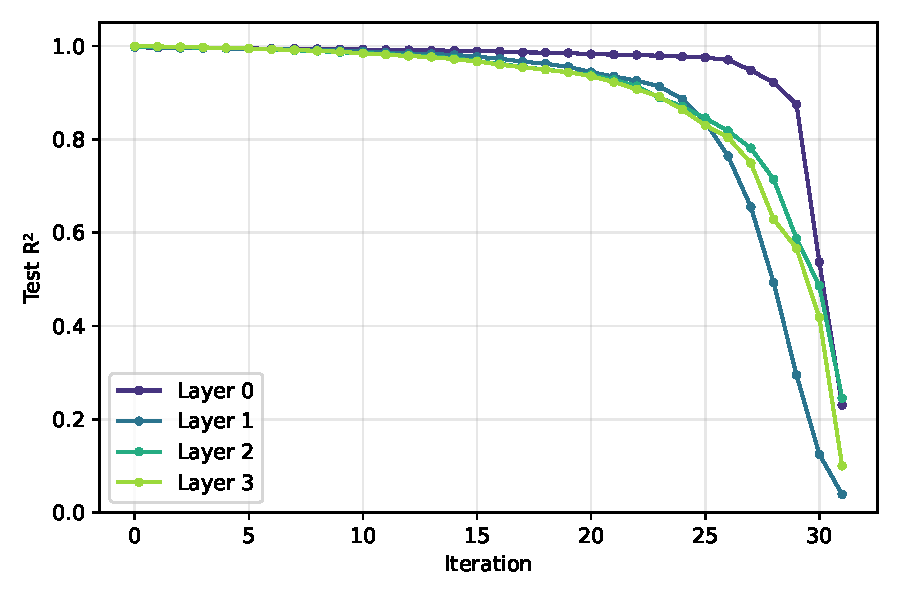
\includegraphics[width=0.7\textwidth]{r2_vs_iteration}
  \caption{Test $R^2$ as a function of iteration for each layer.  Even after 10 rounds of projection, $R^2$ remains above 0.98 at all layers.}
  \label{fig:r2}
\end{figure}

Figure~\ref{fig:r2} shows the central finding: \textbf{all four layers sustain $R^2 > 0.98$ across all 10 iterations}.  The algorithm never triggers the $R^2 < 0.05$ stopping criterion.  Each iteration extracts a rank-2 subspace (consistent with the 2D simplex geometry of the Mess3 belief state), so 10 iterations consume $10 \times 2 = 20$ of the 64 available dimensions.

This means the belief state can be linearly decoded from at least 10 mutually orthogonal 2D subspaces within each layer's residual stream.  The $R^2$ drop from iteration 0 to iteration 9 is modest: 0.0045 at layer 0, increasing to 0.013 at layer 3.

\begin{figure}[ht]
  \centering
  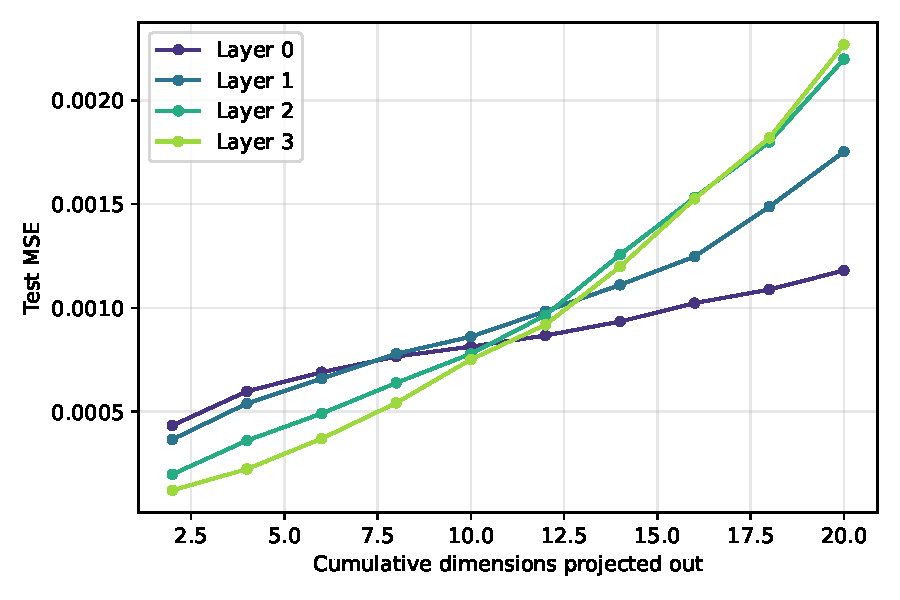
\includegraphics[width=0.7\textwidth]{mse_vs_dims}
  \caption{Test MSE increases approximately linearly with the number of dimensions projected out, but remains small relative to the target variance.}
  \label{fig:mse}
\end{figure}

Figure~\ref{fig:mse} shows the corresponding MSE growth.  Later layers start with lower MSE (layer 3 begins at $1.2 \times 10^{-4}$, vs.\ $4.3 \times 10^{-4}$ for layer 0), reflecting a more precise belief-state encoding deeper in the network.  The MSE growth is approximately linear in the number of removed dimensions, suggesting that the redundant copies contribute roughly equally to probe accuracy.

\subsection{Counterfactual Importance: A Strong Hierarchy}

\begin{figure}[ht]
  \centering
  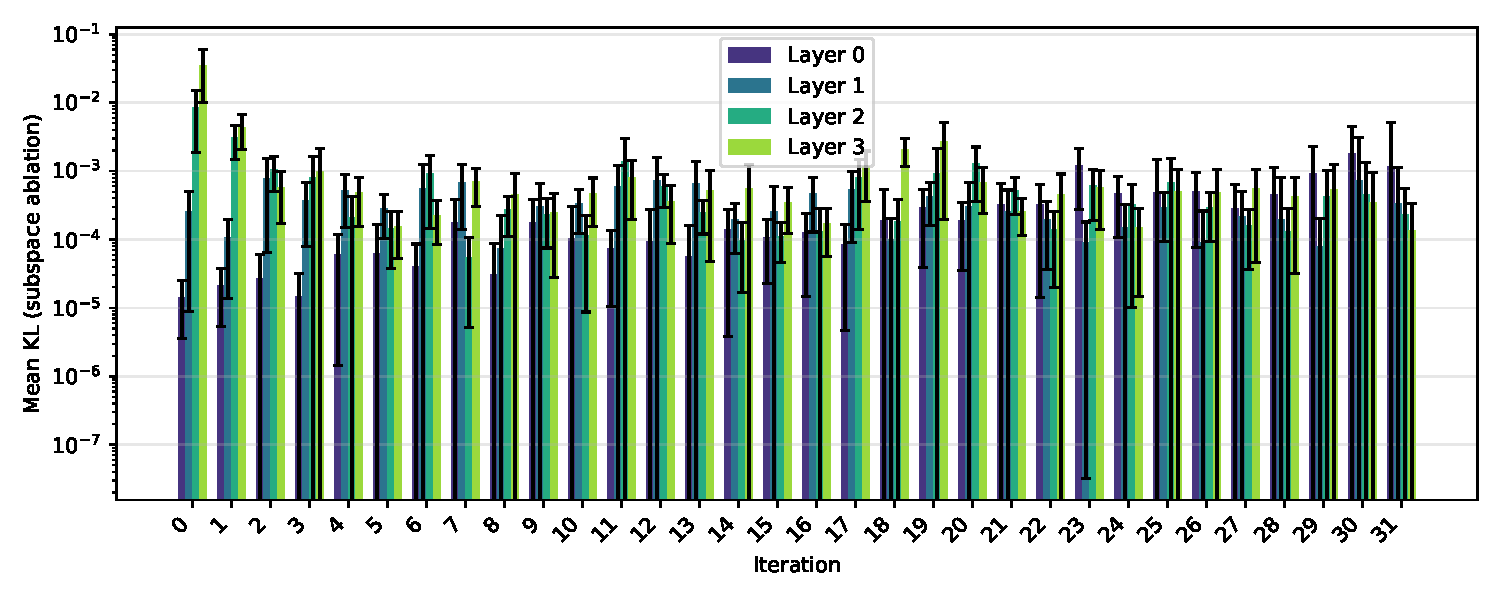
\includegraphics[width=0.85\textwidth]{kl_per_iteration}
  \caption{Mean KL divergence from ablating each iteration's subspace, broken down by layer.  Note the log scale.  Iteration 0 at layer 3 dominates.}
  \label{fig:kl-iter}
\end{figure}

Figure~\ref{fig:kl-iter} reveals a strikingly different picture from the probing results.  While all 10 subspaces are equally \emph{decodable}, they are far from equally \emph{important}:

\begin{itemize}
  \item \textbf{Layer 3, iteration 0} produces the largest KL shift by a wide margin: $\text{KL} = 0.039 \pm 0.027$.  The second iteration at layer 3 drops by nearly 10$\times$ to $\text{KL} = 0.004$.
  \item \textbf{Layer 0} subspaces are almost entirely causally inert: even the cumulative ablation of all 20 dimensions yields KL $= 0.003$.  This suggests that the belief-state information in the early residual stream, while decodable, is not used by the model for prediction at the output.
  \item The causal importance follows a clear \textbf{layer hierarchy}: layer 3 $\gg$ layer 2 $>$ layer 1 $\gg$ layer 0.
\end{itemize}

\begin{figure}[ht]
  \centering
  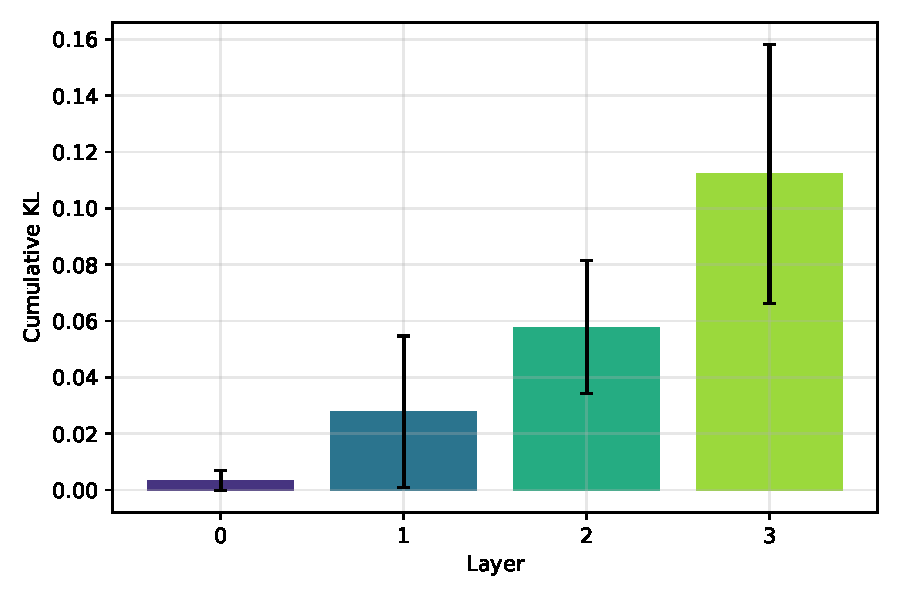
\includegraphics[width=0.55\textwidth]{cumulative_kl}
  \caption{KL divergence from ablating the cumulative 20-dimensional subspace at each layer.}
  \label{fig:kl-cum}
\end{figure}

Figure~\ref{fig:kl-cum} confirms this hierarchy.  The cumulative KL grows roughly exponentially across layers: 0.003 (layer 0), 0.028 (layer 1), 0.058 (layer 2), 0.112 (layer 3).

\begin{figure}[ht]
  \centering
  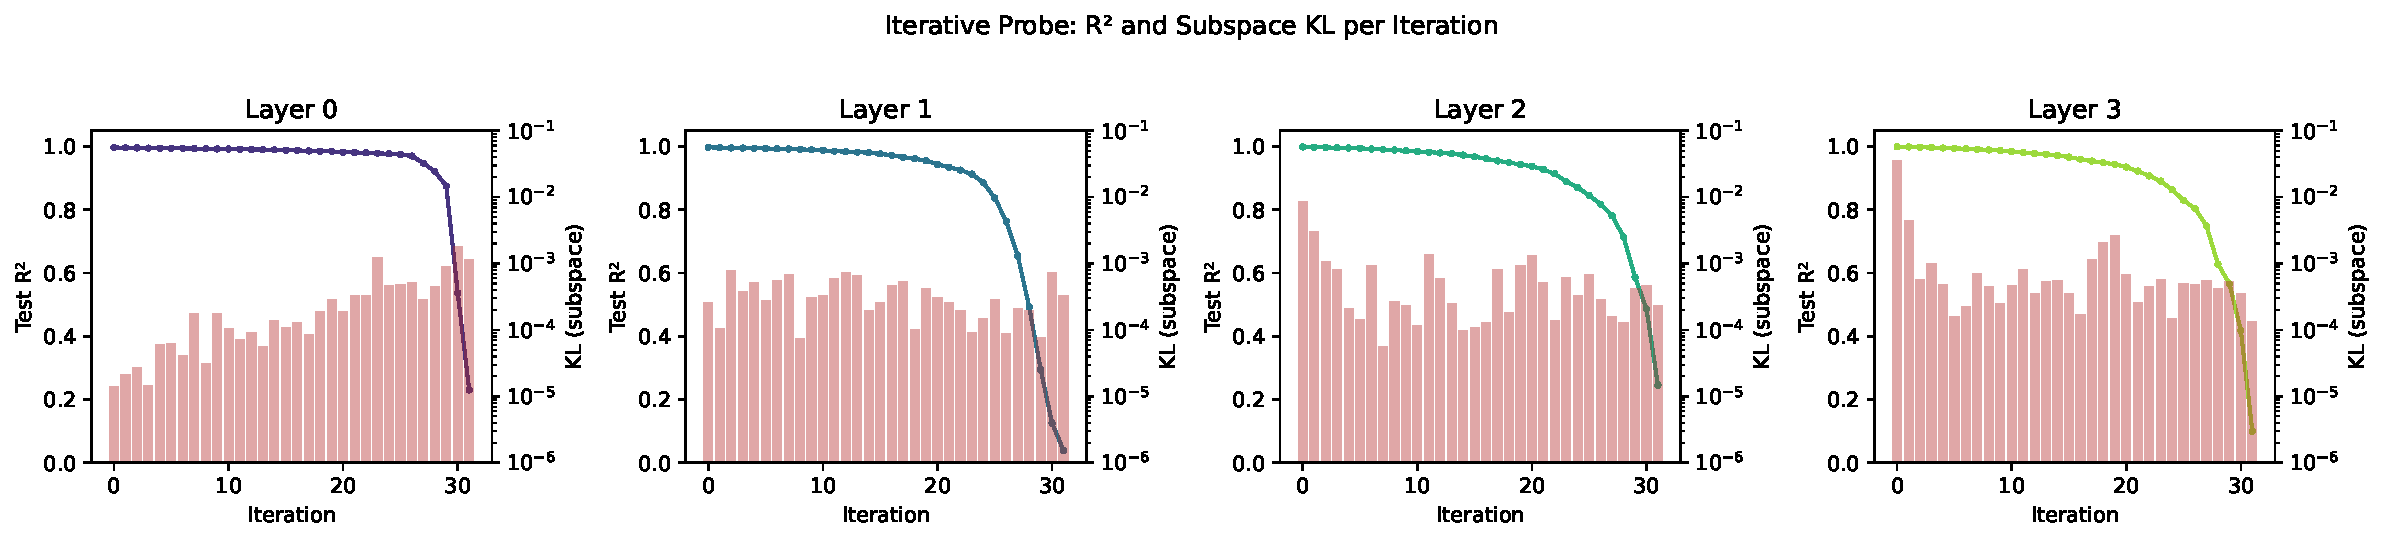
\includegraphics[width=\textwidth]{combined_r2_kl}
  \caption{Dual-axis plots showing decodability ($R^2$, green line) and causal importance (KL, red bars) together for each layer.  The contrast between flat $R^2$ and sharply decaying KL is most pronounced at layer 3.}
  \label{fig:combined}
\end{figure}

Figure~\ref{fig:combined} juxtaposes the two perspectives.  The flat $R^2$ curves and the steeply declining KL bars make the dissociation visually clear: decodability does not imply causal relevance.

%----------------------------------------------------------------------
\section{Discussion}
\label{sec:discussion}
%----------------------------------------------------------------------

\subsection{The Nature of Redundancy}

The fact that the belief state is linearly readable from 10 independent subspaces spanning 20 out of 64 dimensions raises the question: is this deliberate or incidental?

In a linear model, the output logits are computed as $\text{logit} = W_U \, a + b_U$, where $W_U \in \mathbb{R}^{3 \times 64}$ is the unembedding matrix and $a$ is the final residual stream.  The unembedding only ``reads'' the projection of $a$ onto the row space of $W_U$, which is at most 3-dimensional (for a 3-token vocabulary).  In a transformer with nonlinear MLP layers and attention, the situation is more complex: intermediate layers can route information through different subspaces, so multiple copies at an earlier layer may serve different downstream computations.

However, the ablation results suggest that even at the \emph{final} layer, only the first iteration's subspace carries substantial causal weight.  The remaining copies appear to be \textbf{representational byproducts}---linear structure that arises naturally from the network's computation but is not directly utilised for the output.

One plausible mechanism is that each attention head and MLP layer writes a belief-state-correlated component into the residual stream as part of its computation, and these components accumulate across layers.  Since the residual stream is a sum of all layer outputs, any layer that computes a function of the belief state will leave a linearly decodable trace, even if that trace is not read by subsequent layers.

\subsection{Layer Hierarchy and the Residual Stream}

The exponential growth of causal importance across layers (0.003 $\to$ 0.028 $\to$ 0.058 $\to$ 0.112) aligns with the standard picture of transformer computation: early layers build up representations that are progressively refined, and the final layer's output is what directly determines predictions.

The near-zero causal importance of layer 0's belief-state subspace is particularly striking.  The model encodes the belief state with $R^2 = 0.997$ at layer 0, yet ablating all 20 belief-state-correlated dimensions barely affects the output.  This means the subsequent layers do not read the belief state from the directions where a linear probe finds it at layer 0.  They may instead reconstruct it through attention and MLP operations, or read it from entirely different (nonlinear) features of the early residual stream.

\subsection{Decodability $\neq$ Causal Use}

This experiment provides a concrete demonstration of a well-known but often underappreciated point in mechanistic interpretability: \textbf{the existence of a linear probe does not establish causal relevance}.  All 40 subspaces across 4 layers and 10 iterations have $R^2 > 0.98$, yet their KL divergences span nearly four orders of magnitude (from $10^{-5}$ to $10^{-2}$).

The iterative probing methodology makes this dissociation quantitative.  It allows us to say not just ``the belief state is decodable'' but ``the belief state is decodable from $N$ independent subspaces, of which only the first at layer $L$ is causally important.''

\subsection{Comparison to Superposition}

In the superposition literature, networks are known to store more features than they have dimensions by encoding features in nearly-orthogonal directions.  The pattern here is different: the same 2D feature (the belief state) is stored in many exactly-orthogonal copies.  This is closer to \textbf{redundancy} than superposition.

One interpretation is that this redundancy is an artefact of overparameterisation: the network has 64 dimensions but only needs $\sim$2 to represent the belief state, so the gradient-based optimisation naturally distributes belief-state-correlated structure across many directions.  The ablation results suggest that the model has not learned to ``clean up'' this redundancy---it uses a specific 2D subspace and ignores the rest.

%----------------------------------------------------------------------
\section{Implementation Notes}
\label{sec:implementation}
%----------------------------------------------------------------------

The implementation is split across two files:

\begin{itemize}
  \item \code{src/iterative\_probe.py}: Pure numpy/sklearn logic for the iterative probing algorithm.  Contains the dataclasses \code{IterationResult} and \code{IterativeProbeResult}, and the functions \code{extract\_subspace()}, \code{project\_out\_subspace()}, \code{iterative\_probe\_single\_layer()}, and \code{iterative\_probe\_all\_layers()}.
  \item \code{src/run\_iterative\_probe.py}: CLI pipeline that orchestrates data generation, activation extraction (reusing \code{src/activation\_extraction.py}), iterative probing (Phase 1), and counterfactual ablation (Phase 2).  The ablation helpers \code{ablate\_subspace()} and \code{compute\_counterfactual()} are defined here.
\end{itemize}

The CLI supports \code{-{}-skip-counterfactual} for running Phase 1 alone, and \code{-{}-force} to re-run over existing results.  Output is saved to \code{\{model\_dir\}/iterative\_probe\_results/} as three files: \code{iterative\_metrics.csv}, \code{counterfactual\_metrics.csv}, and \code{subspaces.npz}.

%----------------------------------------------------------------------
\section{Conclusion}
\label{sec:conclusion}
%----------------------------------------------------------------------

Iterative probing reveals that a 4-layer, 64-dimensional transformer trained on the Mess3 HMM stores the 2D belief state in at least 10 mutually orthogonal subspaces at every layer, consuming 20 of 64 dimensions.  Despite this extensive redundancy, counterfactual ablation shows that only the first subspace at the final layer carries substantial causal weight for next-token prediction.

This dissociation between decodability and causal importance has methodological implications: probe $R^2$ alone is insufficient for understanding which representations a network actually relies upon.  The iterative probing framework provides a structured way to quantify both the degree of redundancy and the causal hierarchy among redundant copies.

\end{document}
